\documentclass[../../Cours_M1.tex]{subfiles}

\newcommand{\nomTD}{TP1 : Synthèse et réalisation de filtres actifs}
\renewcommand{\nomentete}{UE431 - \nomTD}
\renewcommand{\auteur}{Aymeric Arnould, Tom Colinot}

\title{\nomTD}
\author{\auteur}

\renewcommand{\thesubsection}{\Roman{subsection}.}

\begin{document}

\maketitle

\section*{Préparation}

\subsection{Mesure automatique du diagramme de Bode}
\begin{itemize}
\item On donne une fréquence maximale $f_{max}$, une fréquence minimale $f_{min}$ et un nombre de points $N$ et on désire générer une répartition logarithmique de ces points.

Ainsi, on a pour le $n$-ème point :
\begin{align*}
\log(f_n) & = \log(f_{min}) + \frac{\log(f_{max})-\log(f_{min})}{N} \\
f_n & = f_{min}(\frac{f_{max}}{f_{min}})^{n/N}
\end{align*}

\item Pour obtenir un fonctionnement correct des filtres à amplificateurs opérationnels, il faut veiller à ce que $2\pi f A_s < SR$, où $A_s$ est l'amplitude de sortie de l'AO.

\item Pour effectuer le tracé du diagramme de Bode point par point, on génère une tension sinusoïdale d'amplitude $V_e$ pour chacune des fréquences $f_n$ réparties logarithmiquement sur l'intervalle choisi $[f_{min},f_{max}]$ choisi.
On mesure pour chacune de ces  fréquences l'amplitude $V_s$ du signal de sortie, et on trace le gain $G=20\log(V_s/V_e)$ en fonction de $f_n$. On ne mesure pas le déphasage car le cahier des charges n'impose pas de contrainte sur la phase.
\end{itemize}

\subsection{Synthèse d'un filtre passe-bas de Butterworth}

\paragraph{Gabarit} On désire réaliser un filtre passe-bas de Butterworth admettant :
\begin{itemize}
\item une bande passante $f_p = 4,5kHz$ avec un gain $a=-3dB$
\item un gain maximal $b=-35dB$ pour des fréquences supérieures à $f_a = 13kHz$
\end{itemize}

\begin{figure}[h!]
\centering
\begin{tikzpicture}[scale=1]
\draw [>=latex,->] (0,0) node[left]{0} -- (8,0) node[right]{$f$} ;
\draw [>=latex,->] (0,-3) -- (0,1) node[left]{$G_{dB}$};

\draw [dashed] (0,-2) node[left]{$b=-35dB$} -- (3,-2) -- (3,0) node[above]{$f_p=4,5kHz$};
\draw [dashed] (3,-2) -- (6,-2);
\draw (0,-1) node[left]{$a=-3dB$} -- (3,-1) -- (3,-3);
\draw (6,0) node[above]{$f_a=13kHz$} -- (6,-2) -- (8,-2);
\end{tikzpicture}
\caption{Gabarit du filtre passe bas}
\end{figure}

\paragraph{Sélectivité} La sélectivité du filtre correspond à $k= \frac{f_p}{f_a} =  0,35$.

\paragraph{Fonction d'approximation d'un filtre de Butterworth}
\[H^2(j\Omega) = \frac{1}{1+\epsilon^2\Omega^{2n}} \avec \Omega = \frac{f}{f_p}\]


\begin{align*}
\intertext{Déterminons l'expression de $\epsilon$ en fonction de $a$.}
\text{Par définition } a & = 20 \log(H(j\Omega))|_{\Omega=1} \\
& = 10 \log \frac{1}{1+\epsilon^2} \\
10^{-\frac{a}{10}} & = 1 + \epsilon^2 \\
\text{donc } & \boxed{\epsilon = \sqrt{10^{-\frac{a}{10}}-1}} \\
\text{On a donc } & \epsilon = 1 \text{ pour } a = -3 dB
\intertext{Déterminons ensuite l'expression de l'ordre minimal $n_{min}$ du filtre passe-bas normalisé.}
\text{Par définition } b & = 20 \log(H(j\Omega))|_{\Omega=\Omega_a=1/k} \\
& = 10 \log (\frac{1}{1+\epsilon^2k^{-2n}})\\
10^{-\frac{b}{10}} & = 1 + \epsilon^2 k^{-2n} \\
k^{-2n} & = \frac{10^{-\frac{b}{10}}-1}{\epsilon^2} \\
\text{donc } & \boxed{n = \frac{\ln (\frac{10^{-\frac{b}{10}}-1}{\epsilon^2})}{2\ln(\frac{1}{k})}} \\
& n \approx 3,84 \text{ pour } b = -35dB, k = 0,35\\
\text{On a donc } & n_{min} = 4
\end{align*}

\paragraph{Calcul de la fonction de transfert normalisée $H(s)$ du filtre passe-bas prototype}

\begin{align*}
H(s) & = \frac{1}{\sqrt{1+\epsilon^2(-1)^ns^{2n}}} \avec s = p/\omega_p\\
H^2(s) & = \frac{1}{1+s^8} \text{ avec } n=4
\end{align*}

On détermine $H$ à partir des racines du dénominateur de $H^2$ dont on ne garde que celles à partie réelle strictement négative.

\[1+s^8 = 0 \Leftrightarrow s = e^{j\frac{2k+1}{8}\pi} k=0,..7 \]

Les racines à partie réelle strictement négative sont $e^{j\frac{5\pi}{8}},e^{j\frac{7\pi}{8}},e^{-j\frac{5\pi}{8}},e^{-j\frac{7\pi}{8}}$

\begin{align*}
H(s) & = \frac{1}{(s-e^{j\frac{5\pi}{8}})(s-e^{j\frac{7\pi}{8}})(s-e^{-j\frac{5\pi}{8}})(s-e^{-j\frac{7\pi}{8}})} \\
& = \frac{1}{(s^2-s(e^{j\frac{5\pi}{8}}+e^{-j\frac{5\pi}{8}})+1)(s^2-s(e^{j\frac{7\pi}{8}}+e^{-j\frac{7\pi}{8}})+1)} \\
& = \frac{1}{(s^2-2s\cos(\frac{5\pi}{8})+1)(s^2-2s\cos(\frac{7\pi}{8})+1)} \\
\text{donc } & \boxed{H(s) = \frac{1}{(s^2+0,7654s+1)(s^2+1,8478s+1)}} \\
\end{align*}

On retrouve bien ce résultat dans le tableau B1 pour un filtre passe-bas d'ordre 4.


\subsection{Synthèse d'un filtre passe-bas de Tchebychev}

Un filtre passe-bas de Tchébychev est caractérisé par la fonction d'approximation suivante :

\[ F(\Omega) = \frac{1}{1+\epsilon^2T_a^2(\Omega)} \avec \begin{array}{ll}
Ta(\Omega) = \cos[n.\arccos(\Omega)] & \Omega \leq 1 \\
Ta(\Omega) = \cosh[n.\argch(\Omega)] & \Omega < 1
\end{array}
\et \Omega = \frac{f}{f_p}
\]

Déterminons l'expression de $\epsilon$ en fonction de $a$.
\begin{align*}
\text{Par définition } a & = 20 \log(F(\Omega))|_{\Omega=1}  \\
\text{Comme précédemmment, } \epsilon & = \sqrt{10^{-\frac{a}{10}}-1}
\end{align*}

Pour déterminer l'ordre minimal du filtre $n_{min}$, on utilise le point de coordonnées $(\Omega_a=\frac{1}{k},b)$ :
\begin{align*}
\text{Par définition, } b & = 10\log(\frac{1}{1+\epsilon^2T_n^2(\Omega_a)}) \\
10^{-\frac{b}{10}} & = 1 + \epsilon^2T_n^2(\Omega_a) \\
T_n^2(\Omega_a) & = \frac{10^{-\frac{b}{10}}-1}{\epsilon^2}
\intertext{Comme $\Omega_a=1/k \approx 2.857 >1$, alors }
T_n^2(\Omega_a)& = \cosh(n\argch(\Omega_a)) \\
n & = \frac{\argch(\frac{\sqrt{10^{-\frac{b}{10}}-1}}{\epsilon^2})}{\argch(\Omega_a)}
\end{align*}
Avec $\epsilon = 1$, $b=-35dB$, et $\Omega_a = \frac{1}{0,35}=2,857$, on obtient
\[ n = 2,76 \text{ donc } n_{min} = 3\]

\paragraph{Fonction de transfert}
On souhaite réaliser un filtre avec les mêmes caractéristiques que précédemment mais avec une ondulation dans la bande passante limitée à $a=-1dB$. Il faudra donc augmenter l'ordre par rapport au filtre déterminé ci-dessus.

Pour un filtre d'ordre 4, on aura la fonction de transmission suivante :
\[ \boxed{ H(s) = \frac{1}{(1,0136s^2 + 0,2828s +1)(3,5791s^2 + 2,4113s+1)} \avec s = \frac{p}{\omega_p} }\]


\subsection{Réalisation des filtres passe-bas}

\subsubsection{La structure de Sallen-Key}

Pour réaliser les filtres passe-bas cascadables, il est intéressant d'utiliser des amplificateurs opérationnels qui fournissent des filtres à grande impédance d'entrée et faible impédance de sortie. On utilise ici la structure de Sallen-Key.

\begin{figure}[h!]
\centering
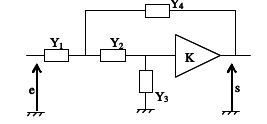
\includegraphics[scale=0.6]{sk.png}
\caption{Structure de Sallen-Key}
\end{figure}

On note $u_K$ la tension en entrée de l'amplificateur de tension, on a alors $s = Ku_K$.

L'application du théorème de Millman au point A situé entre $Y_1$, $Y_2$ et $Y_4$ donne :

\[V_A = \frac{Y_1e + Y_2u_K + Y_4s}{Y_1+Y_2+Y_4} = \frac{Y_1e + Y_2\frac{s}{K} + Y_4s}{Y_1+Y_2+Y_4}\]

En entrée de l'amplificateur de tension, supposé idéal, le courant est quasi-nul donc on a un diviseur de tension :
\[u_K = \frac{Y_2}{Y_2 + Y_3} V_A =\frac{s}{K}\]

Ainsi, on en déduit :
\begin{align*}
\frac{Y_1}{Y_1+Y_2+Y_4}e & = (-\frac{\frac{Y_2}{K}+Y_4}{Y_1+Y_2+Y_4} + \frac{Y_2+Y_3}{Y_2K})s \\
e & = (-\frac{\frac{Y_2}{K}+Y_4}{Y_1} + \frac{(Y_2+Y_3)(Y_1+Y_2+Y_4)}{Y_1Y_2K})s \\
e & = (\frac{(Y_2+Y_3)(Y_1+Y_4)}{KY_2} + \frac{Y_2+Y_3}{K}-\frac{Y_2}{K}-Y_4)\frac{s}{Y_1} \\
\frac{s}{e} & = \frac{KY_1Y_2}{(Y_2+Y_3)(Y_1+Y_4)+Y_2(Y_3-KY_4)}
\end{align*}

Pour réaliser l'amplificateur de tension parfait de gain K, on réalise le montage suivant :

\begin{figure}[h!]
\centering
\begin{tikzpicture}{scale=0.5}
\draw
(4,1.5) node[op amp] (opamp) {}
(0,0) node[ground]{} -- (0,2)   to[R,l=$r_1$] (2,2) -- (opamp.-)
(2,2) -- (2,3) to [R,l=$r_2$] (5,3) -- (5,1.5)
(opamp.+) node[left]{$u_K$}
(opamp.out) -- (6,1.5) node[right]{$s$}
;
\end{tikzpicture}
\end{figure}

On a $V_-=V_+$ et $V_- = \frac{r_1}{r_1+r_2} s$, d'où $u_K=\frac{r_1}{r_1+r_2}s $ donc le gain $K$ est défini par $K=1+\frac{r_2}{r_1}$

On pose alors $Y_1 = \frac{1}{R_1}$, $Y_2=\frac{1}{R_2}$, $Y_3 = C_3p$ et $Y_4=C_4p$.

\[ H_{SK}(p) = \frac{K}{R_1C_3R_2C_4p^2 + (R_1(C_3+(1-K)C_4)+R_2C_3)p+1} \]

On a donc
\begin{eqnarray*}
H_{SK}(p) = \frac{K}{(\frac{p}{\omega_0})^2 + 2m\frac{p}{\omega_0}+1} \quad \avec \quad & \omega_0^2 & = \frac{1}{R_1C_3R_2C_4} \\
& m & = \frac{(R_1(C_3+(1-K)C_4)+R_2C_3)}{2\sqrt{R_1C_3R_2C_4}}
\end{eqnarray*}

\noindent Comme $K$ intervient dans l'expression de $m$ et non dans celle de $\omega_0$, on peut régler indépendamment ces deux paramètres. Pour régler $m$ uniquement, on peut utiliser une résistance variable ($r_1$ ou $r_2$) pour faire varier $K$.

\subsubsection{Réalisation du filtre passe-bas de Butterworth}

On pose $R_1=R_2=R$ et $C_3=C_4=C$, on a :
\[ H_{SK}(p) = \frac{K}{R^2C^2p^2 + RC(3-K)p+1} \]
\[ H_{SK}(s) = \frac{K}{R^2C^2\omega_p^2s^2 + RC(3-K)\omega_ps+1} \]

Or, on doit synthétiser :
\[H(s) = \frac{1}{(s^2+0,7654s+1)(s^2+1,8478s+1)}\]

Circuit 1 :\\
\[H_{SK}(s) = \frac{K}{R^2C^2\omega_p^2s^2 + RC(3-K)\omega_ps+1} = \frac{1}{(s^2+0,7654s+1)}\]
\[
\left\{
\begin{array}{ll}
R^2C^2\omega_p^2 & = 1\\
RC(3-K)\omega_p & = 0,7654 \\
C & = 4,7nF
\end{array}
\right.
\rightarrow
\left\{
\begin{array}{ll}
R & = 7525 \Omega\\
K & = 2,2346 \\
C & = 4,7nF
\end{array}
\right.
\]

Circuit 2 :\\
\[H_{SK}(s) = \frac{K}{R^2C^2\omega_p^2s^2 + RC(3-K)\omega_ps+1} = \frac{1}{(s^2+1,8478s+1)}\]
\[
\left\{
\begin{array}{ll}
R^2C^2\omega_p^2 & = 1\\
RC(3-K)\omega_p & = 1,8478  \\
C & = 4,7nF
\end{array}
\right.
\rightarrow
\left\{
\begin{array}{ll}
R & = 7525 \Omega\\
K & = 1,1522 \\
C & = 4,7nF
\end{array}
\right.
\]

Par choix des valeurs de $K$ dans chacun des circuits, la valeur du gain global ne sera pas unitaire. Si on veut un gain unitaire, il faudra rajouter un étage amplificateur ou atténuateur.

\subsubsection{Réalisation du filtre passe-bas de Tchebychev}

Si $K=2$ et $C_3=C_3=C$, alors on a
\[H_{SK}(p) = \frac{K}{R_1R_2C^2p^2 + R_2Cp+1}\]

La valeur de $K=2$ permet donc de simplifier les équations conduisant aux valeurs des paramètres.
On voulait synthétiser :
\[H(s) = \frac{1}{(1,0136s^2 + 0,2828s +1)(3,5791s^2 + 2,4113s+1)} \avec s = \frac{p}{\omega_p}\]

Circuit 1:\\
\[H_{SK}(s) = \frac{K}{R_1R_2C^2\omega_p^2s^2+R_2C\omega_ps+1}
=\frac{1}{(1,0136s^2 + 0,2828s +1)}\]
\[
\left\{
\begin{array}{ll}
R_1R_2C^2\omega_p^2 & = 1,0136 \\
R_2C\omega_p & = 0.2828 \\
C & = 4,7 nF
\end{array}
\right.
\rightarrow
\left\{
\begin{array}{ll}
R_1 & = 26,98k\Omega \\
R_2 & = 2,13 k\Omega \\
C & = 4,7 nF
\end{array}
\right.
\]

Circuit 2:\\
\[H_{SK}(s) = \frac{K}{R_1R_2C^2\omega_p^2s^2+R_2C\omega_ps+1}
=\frac{1}{(3,5791s^2 + 2,4113s +1)}\]
\[
\left\{
\begin{array}{ll}
R_1R_2C^2\omega_p^2 & = 3,5791 \\
R_2C\omega_p & = 2,4113 \\
C & = 4,7 nF
\end{array}
\right.
\rightarrow
\left\{
\begin{array}{ll}
R_1 & = 11,17k\Omega \\
R_2 & = 18,15k\Omega \\
C & = 4,7 nF
\end{array}
\right.
\]

On avait \[m = \frac{(R_1(C_3+(1-K)C_4)+R_2C_3)}{2\sqrt{R_1C_3R_2C_4}} = \frac{(R_1(2-K) + R_2)C}{2\sqrt{R_1R_2C^2}}\]

La valeur de $K_{lim}$ conduisant à un coefficient d'amortissement $m$ négatif est $K_{lim} = 2+ \frac{R_2}{R_1}$.\\

Pour le circuit 1, $K_{lim} = 2 + \frac{2,13}{26,98} = 2,08$.

Pour le circuit 2, $K_{lim} = 2 + \frac{18,15}{11,15} = 3,62$.\\

Comme on a choisi $K=2$, on a $K\approx K_{lim}$ pour le circuit 1.

Il faut déterminer un autre jeu de valeurs avec $C_3=C_4=C$ et $R_1=6,8k\Omega$.

\[H_{SK}(s) = \frac{K}{R_1R_2C^2\omega_ps^2+(R_1(2-K)+R_2)C\omega_ps + 1} = \frac{1}{(1,0136s^2 + 0,2828s +1)}\]
On a donc finalement pour le circuit 1 :
\[
\left\{
\begin{array}{ll}
R_1R_2C^2\omega_p^2 & = 1,0136 \\
(R_1(2-K)+R_2)C\omega_p & = 0.2828 \\
C & = 4,7 nF \\
R_1 & = 6,8k\Omega
\end{array}
\right.
\rightarrow
\left\{
\begin{array}{ll}
R_1 & = 6,8k\Omega \\
R_2 & = 8,4k\Omega \\
C & = 4,7 nF\\
K & = 2,9
\end{array}
\right.
\]
et pour le circuit 2 :
\[H_{SK}(s) = \frac{K}{R_1R_2C^2\omega_p^2s^2+R_2C\omega_ps+1}
=\frac{1}{(3,5791s^2 + 2,4113s +1)}\]
\[
\left\{
\begin{array}{ll}
R_1R_2C^2\omega_p^2 & = 3,5791 \\
R_2C\omega_p & = 2,4113 \\
C & = 4,7 nF
\end{array}
\right.
\rightarrow
\left\{
\begin{array}{ll}
R_1 & = 11,17k\Omega \\
R_2 & = 18,15k\Omega \\
C & = 4,7 nF
\end{array}
\right.
\]

\section*{Expérimentation}
\setcounter{subsection}{0}

\subsection{Étude des filtres en simulation}

\begin{enumerate}

\item Les diagrammes de Bode des filtres de Butterworth et de Tchébychev simulés avec le logiciel sont donnés respectivement en annexes 1 et 2.

Avec les valeurs des composants choisis, on retrouve les caractéristiques attendues : fréquence de coupure à -3dB de 4,5kHz, gain de -35dB à 13kHz.

Les deux filtres respectent les gabarits imposés.

\item Dans les deux cas, le gain à basse fréquence n'est pas unitaire (à cause de la synthèse des filtres), mais on peut toujours rajouter un filtre atténuateur pour diminuer le gain.

Les deux filtres ont globalement même comportement, mais le filtre de Tchébychev comporte une légère ondulation du gain avant la coupure à -3dB.

\item Dans le cas du filtre de Tchébychev,  la dispersion des composants, et notamment de la valeur de $K$, est plus importante que pour un filtre de Butterworth. L'augmentation de la valeur de $K$ crée une ondulation plus importante en basse fréquence, surtout si on se rapproche de valeur limite d'instabilité $K_{lim}$.
\end{enumerate}

\subsection{Filtre passe-bas de Butterworth}

\begin{enumerate}
\item Pour régler le gain de chaque circuit, on se place à très basse fréquence $f=1Hz$. En visualisant l'entrée et la sortie d'un seul circuit, on peut ajuster le gain : on règle $R_2$, qui est un potentiomètre alors que $R_1$ est fixée, jusqu'à atteindre le gain voulu.
\item Le diagramme de Bode a été relevé dans la partie suivante à l'aide du programme \textit{ScopeWithScopeGen}.
\end{enumerate}

\subsection{Étude des filtres à l'aide du logiciel de programmation graphique}

La partie programmation graphique via l'environnement VEE Pro n'a pas été traitée pendant le TP. Les diagrammes de Bode ont été relevés via \textit{ScopeWithScopeGen}.

\subsubsection{Diagrammes de Bode}
Les diagrammes de Bode sont donnés en annexes 3 et 4.\\

\textit{Filtre de Butterworth :}\\
À basse fréquence, le gain est d'environ 8dB. Lorsque la fréquence augmente, le gain diminue et la limite à -3dB de la bande-passante est atteinte pour une fréquence de 4,5kHz. Le gabarit est bien respecté car on atteint -35dB pour une fréquence de 13kHz.

L'ordre dans lequel sont cascadés les circuits peut avoir une influence. En effet, le circuit 2 présente une résonance. Si on le met en premier, selon l'amplitude du signal d'entrée, la sortie de ce circuit peut saturer l'entrée du circuit suivant : les performances ne seront pas celles attendues. \\

\textit{Filtre de Tchebychev :}\\
À basse fréquence, le gain est d'environ 15dB. Le filtre présente une résonance avant la limite de la bande passante. À 13kHZ, la différence de gain par rapport à la limite basse fréquence est légèrement inférieure au -35dB attendu. Cela est sûrement dû au réglage des gains, car nous avons eu du mal à ajuster les potentiomètres.

\subsubsection{Comparaison des deux filtres passe-bas réalisés}
Les deux filtres ont globalement la même réponse. Cependant, le filtre de Tchebychev présente une résonance à la limite de la bande passante, contrairement au filtre de Butterworth. La pente au-delà de la bande passante du filtre de Tchebychev est plus importante que celle de Butterworth.\\

Les deux filtres ont donc des performances similaires, mais présentent des légères différences qui peuvent justifier l'utilisation de l'un ou de l'autre, selon le cahier des charges imposé.
\end{document}
